\documentclass{article}

% to avoid loading the natbib package, add option nonatbib:
% \usepackage[nonatbib]{style}

\usepackage[final]{style}

\usepackage[utf8]{inputenc} % allow utf-8 input
\usepackage[T1]{fontenc}    % use 8-bit T1 fonts
\usepackage{hyperref}       % hyperlinks
\usepackage{url}            % simple URL typesetting
\usepackage{booktabs}       % professional-quality tables
\usepackage{amsfonts}       % blackboard math symbols
\usepackage{nicefrac}       % compact symbols for 1/2, etc.
\usepackage{microtype}      % microtypography
\usepackage{amsmath}
\usepackage{amssymb}
\usepackage{verbatim}
\usepackage{graphicx}
\usepackage{float}
\usepackage{algorithm}
\usepackage[noend]{algpseudocode}
\newcommand{\argmax}{\arg\!\max}
\DeclareMathOperator{\Rank}{Rank}
\def\BState{\State\hskip-\ALG@thistlm}
\makeatother

\title{Lecture 13: Face Recognition and LDA}

\author{
  \textbf{JR Cabansag, Yuxing Chen, Jonathan Griffin, Dunchadhn Lyons, George Preudhomme} \\
  Department of Computer Science\\
  Stanford University\\
  Stanford, CA 94305 \\
  \texttt{\{cabansag, yxchen28, jgriffi2, dunlyons, gpreud\}@cs.stanford.edu} \\
}

\begin{document}

\maketitle

\section{Introduction to Facial Recognition}
\subsection{Neuroscience Background}
In the 1960's and 1970's, neuroscientists discovered that depending on the angle of observation, certain brain neurons fire when looking at a face. More recently, they have come to believe that an area of the brain known as the \textbf{Fusiform Face Area (FFA)} is primarily responsible for reacting to faces. These advances in the biological understanding of facial recognition have been mirrored by similar advances in computer vision, as new techniques have attempted to come closer to the standard of human facial recognition. 

\subsection{Applications}
Computer facial recognition has a wide range of applications:
\begin{itemize}
  \item \underline{Digital Photography:} Identifying specific faces in an image allows programs to respond uniquely to different individuals, such as centering the image focus on a particular individual or improving aesthetics through various image operations (blur, saturation, etc).
  \item \underline{Surveillance:} By recognizing the faces of specific individuals, we can use surveillance cameras to detect when they enter a location.
  \item \underline{Album Organization:} If we can recognize a specific person, we can group images in which they appear.
  \item \underline{Person tracking:} If we can recognize a specific person, we can track their location through frames of video (useful for surveillance or for robots in the home).
  \item \underline{Emotions and Expressions:} By detecting emotions or facial expressions, we can build smart devices that interact with us based on mood.
  \item \underline{Security and Warfare:} If we can recognize a specific person, we can identify potential threats in drone images and video.
  \item \underline{Teleconferencing:} If we can recognize specific people, then teleconferencing applications could automatically provide information to users about who they are communicating with.
\end{itemize}

\subsection{A Key Distinction: Detection vs. Recognition}
While face \textbf{detection} determines whether an image contains faces and where in the image they are, face \textbf{recognition} determines to \underline{whom} a detected face belongs to (i.e., identifying the identity of the person).

\subsection{Space of Faces}
If we consider an $m \times n$ image of a face, that image can be represented by a point in high dimensional space (${\mathbb{R}}^{mn}$). But relatively few high-dimensional vectors consist of valid face images (images can contain much more than just faces), and thus the region that an arbitrary face image could fall into is a relatively small subspace. The task is to effectively model this subspace of face images.

\begin{figure}[h]
  \centering
  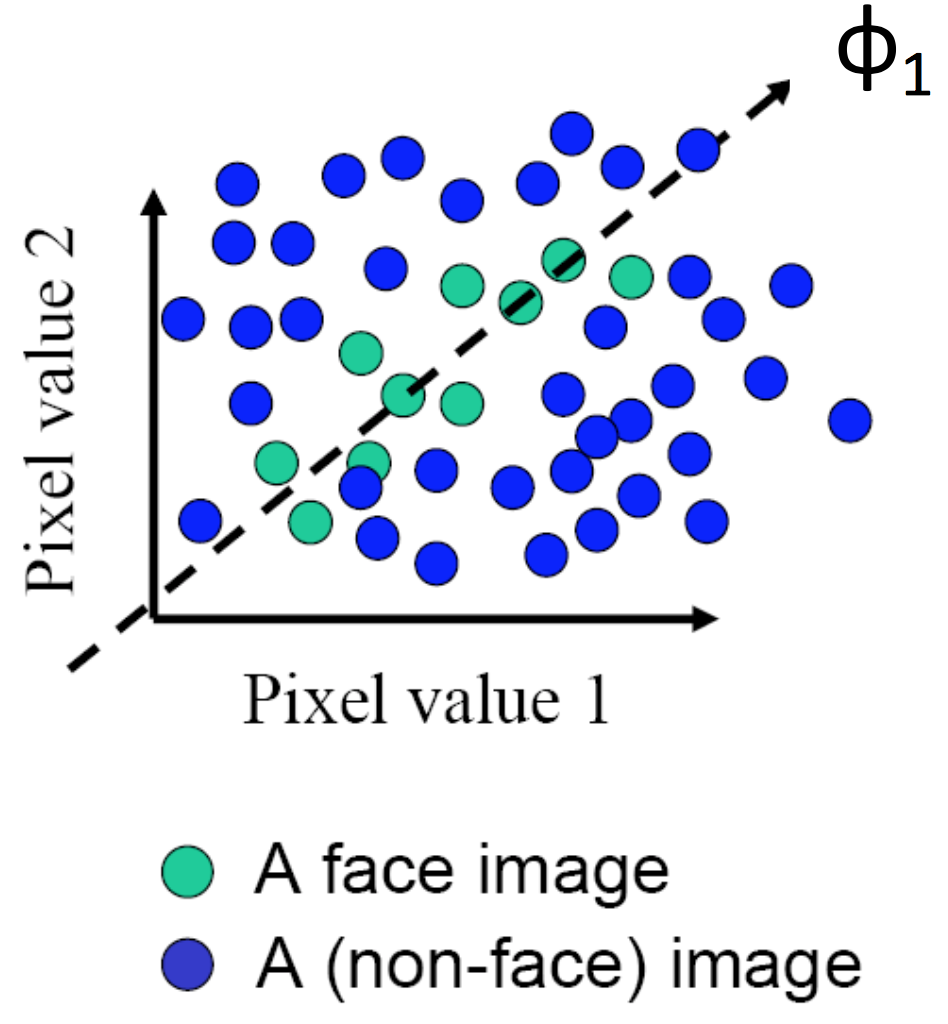
\includegraphics[width=0.55\textwidth]{face_non-face_plot}
  \caption{The region occupied by images of faces is a small subspace of the total space of images. Source: Lecture 13, slide 14}
\end{figure}

In order to model this subspace or "face-space" we compute the k-dimensional subspace such that the projection of the data points onto the subspace has the largest variance among all k-dimensional subspaces. This low-dimensional subspace captures the key appearance characteristics of faces. 

\section{The Eigenfaces Algorithm}

\subsection{Key Ideas and Assumptions}
\begin{itemize}
  \item Assume that most face images lie on a low-dimensional subspace determined by the first $k$ directions of maximum variance.
  \item Use Principle Components Analysis (PCA) to determine the vectors or “eigenfaces” that span that subspace.
  \item Represent all face images in the dataset as linear combinations of eigenfaces, where eigenfaces are defined as the principal components of SVD decomposition.
\end{itemize}

\subsubsection{What are eigenfaces?}
"Eigenfaces" are the visual representations of the eigenvectors in the directions of maximum variance. They often resemble generic-looking faces.
\begin{figure}[h]
  \centering
  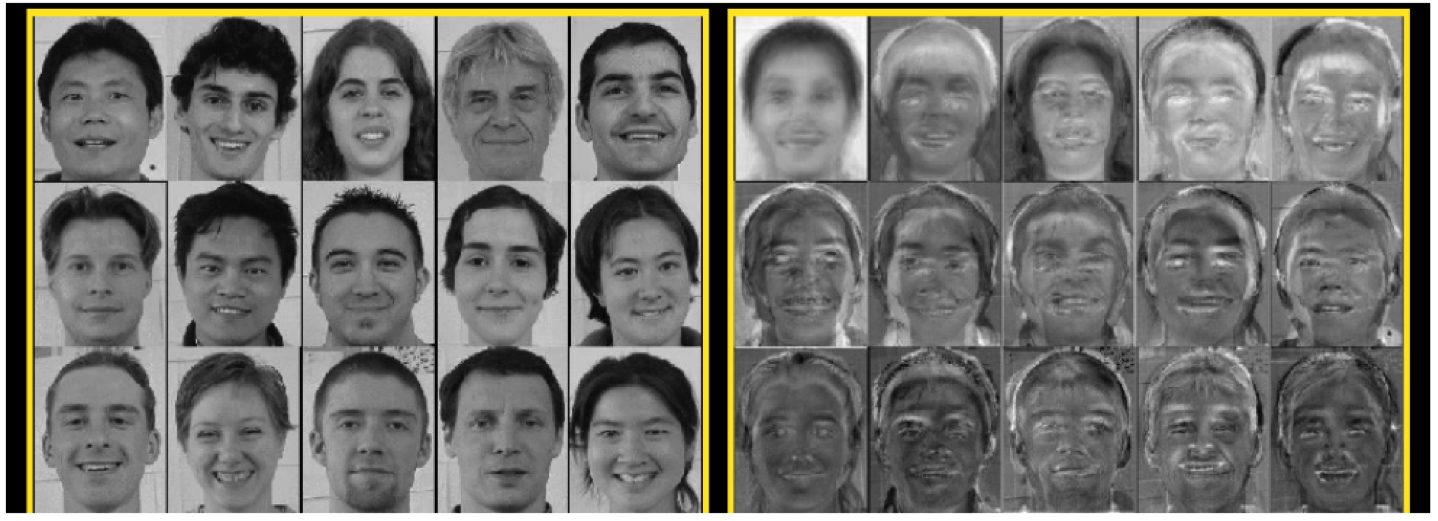
\includegraphics[width=\textwidth]{generic}
  \caption{Faces and Eigenfaces. Source: Lecture 13, slide 29}
\end{figure}

\subsection{Training Algorithm}
\begin{algorithm}[H]
\caption{Eigenfaces Training Algorithm \cite{eigenfaces}}\label{euclid}
\begin{algorithmic}[1]
\State Align training images $x_1, ..., x_n$
\State Compute the average face: 
$$\mu = \frac{1}{N}\sum x_i$$
\State Compute the difference image (the centered data matrix): 
$$X_c = X - \mu 1^{T} = X - \frac{1}{N}X11^{T} = X(1 - \frac{1}{N}11^{T})$$
\State Compute the covariance matrix:
$$\Sigma = \frac{1}{N}X_{c}{X_{c}}^T$$
\State Compute the eigenvectors of the covariance matrix $\Sigma$ using PCA (Principle Components Analysis)
\State Compute each training image $x_{i}$'s projections as 
$$x_i \rightarrow ({x_{i}}^{c} \cdot \phi_{1}, {x_{i}}^{c} \cdot \phi_{2}, ..., {x_{i}}^{c} \cdot \phi_{k}) \equiv (a_1, a_2, ..., a_k)$$
where $\phi_{i}$ is the $i$'th-highest ranked eigenvector
\State The reconstructed face $x_i \approx \mu + a_1 \cdot \phi_1 + ... + a_k \cdot \phi_k$
\end{algorithmic}
\end{algorithm}

\begin{figure}[h]
  \centering
  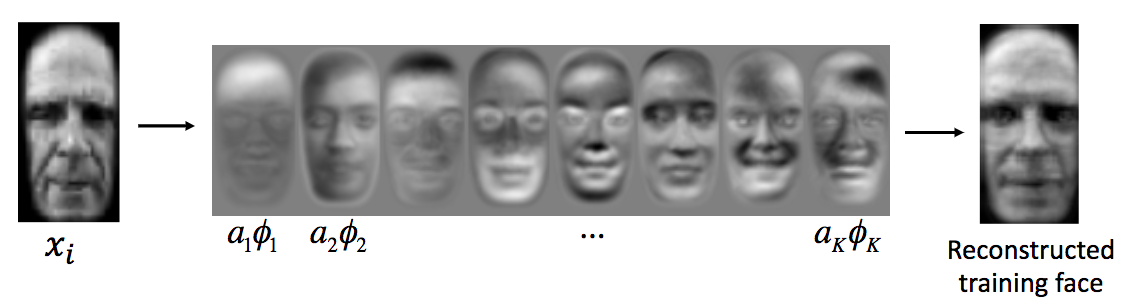
\includegraphics[width=0.8\textwidth]{reconstructed}
  \caption{The reconstructed face after projection. Source: Lecture 13, slide 25}
\end{figure}

\subsubsection{Why can we do this?}
Empirically, the eigenvalues (variance along eigenvectors) drop rapidly with the number of principle components, which is why we can reduce dimensionality without much loss of information.

\begin{figure}[h]
  \centering
  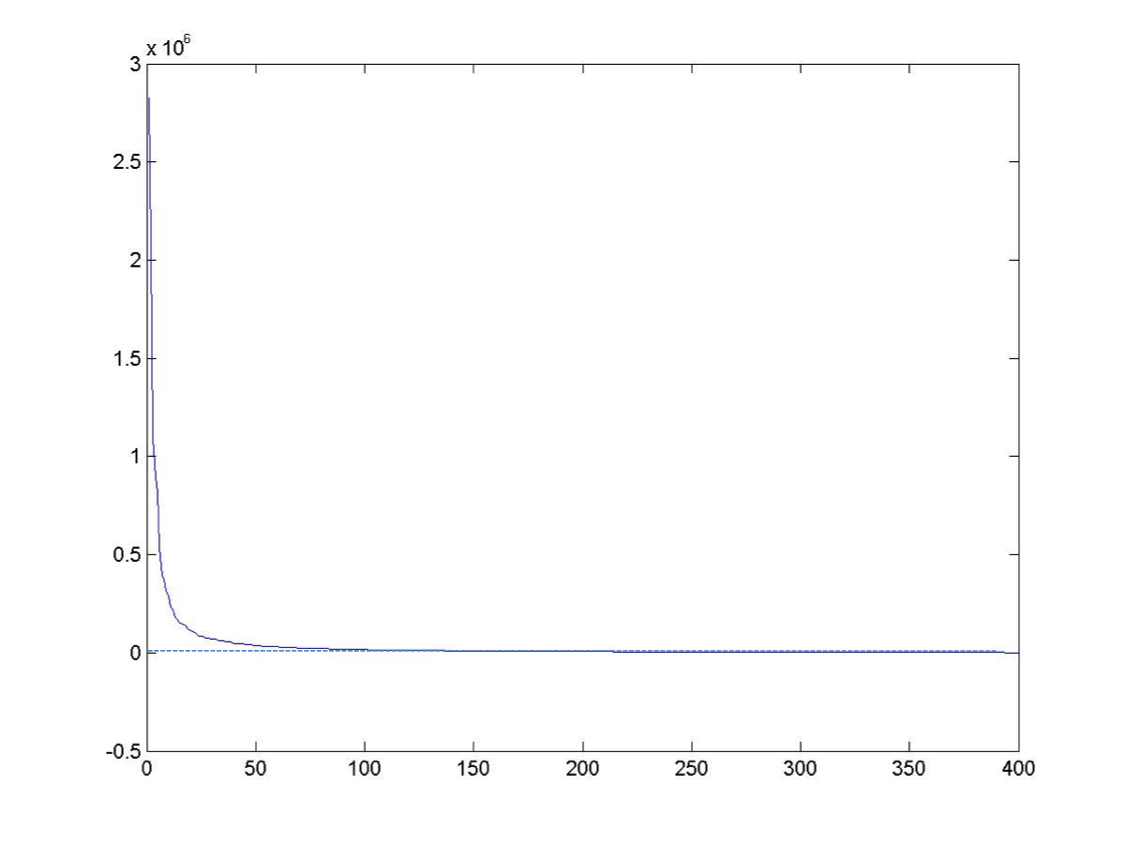
\includegraphics[width=0.7\textwidth]{eigenvalues}
  \caption{Eigenvalues sorted in descending order of magnitude. Source: Lecture 13, slide 26}
\end{figure}

\subsubsection{Reconstruction and Error}
We only select the top $k$ eigenfaces, which reduces the dimensionality. Fewer eigenfaces result in more information loss, and hence less discrimination between faces.

\begin{figure}[h]
  \centering
  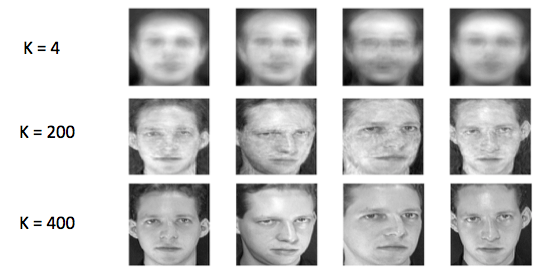
\includegraphics[width=0.55\textwidth]{error}
  \caption{Reconstructed faces with varying number of eigenfaces. Source: Lecture 13, slide 27}
\end{figure}


\subsection{Testing Algorithm}
\begin{algorithm}
\caption{Eigenfaces Testing Algorithm \cite{eigenfaces}}\label{euclid}
\begin{algorithmic}[1]
\State Take query image $t$
\State Project onto eigenvectors:
$$t \rightarrow ((t - \mu) \cdot \phi_{1}, (t - \mu) \cdot \phi_{2}, ..., (t - \mu) \cdot \phi_{k}) \equiv (w_1, w_2, ..., w_k)$$
\State Compare projection $w$ with all $N$ training projections. Use euclidean distance and nearest-neighbors algorithm to output a label
\end{algorithmic}
\end{algorithm}

\subsection{Advantages}
\begin{itemize}
	\item This method is completely knowledge-free -- it does not know anything about faces, expressions, etc.
    \item It is a non-iterative (fast), globally-optimal solution.
\end{itemize}

\subsection{Disadvantages}
\begin{itemize}
	\item This technique requires carefully controlled data.
    \begin{enumerate}
    	\item All faces must be centered in the frame. Otherwise the results may be noisy.
        \item The images must be the same size.
        \item There is some sensitivity to the face angle.
    \end{enumerate}
    \item Method is completely knowledge free.
    \begin{enumerate}
    	\item It makes no effort to preserve class distinctions.
        \item PCA doesn't take into account who it is trying to represent in this lower dimensional space (it doesn't take into account the labels associated with the faces). Therefore, it might map different faces near the same subspace, making it difficult for classifiers to distinguish between them.
    \end{enumerate}
	\item PCA projection is optimal for reconstruction from a low dimensional basis but may not be optimal for discrimination (the algorithm does not attempt to preserve class distinctions).
\end{itemize}

\subsection{Beyond Facial Recognition: Expressions and Emotions}
This technique also generalizes beyond simple facial recognition and can be used to detect expressions and emotions. The subspaces would therefore represent happiness, disgust, or other potential expressions, and the algorithm would remain unchanged. 

\begin{figure}[H]
  \centering
  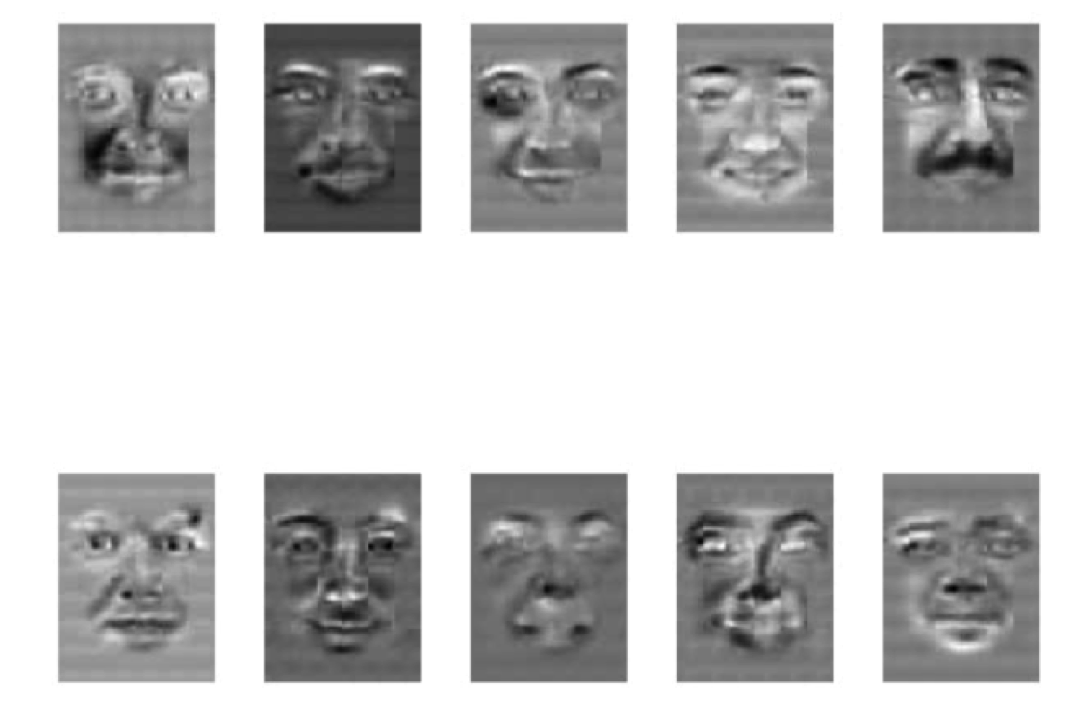
\includegraphics[width=0.65\textwidth]{happy}
  \caption{Eigenfaces expressing happiness. Source: Lecture 13, slide 33}
\end{figure}

\begin{figure}[H]
  \centering
  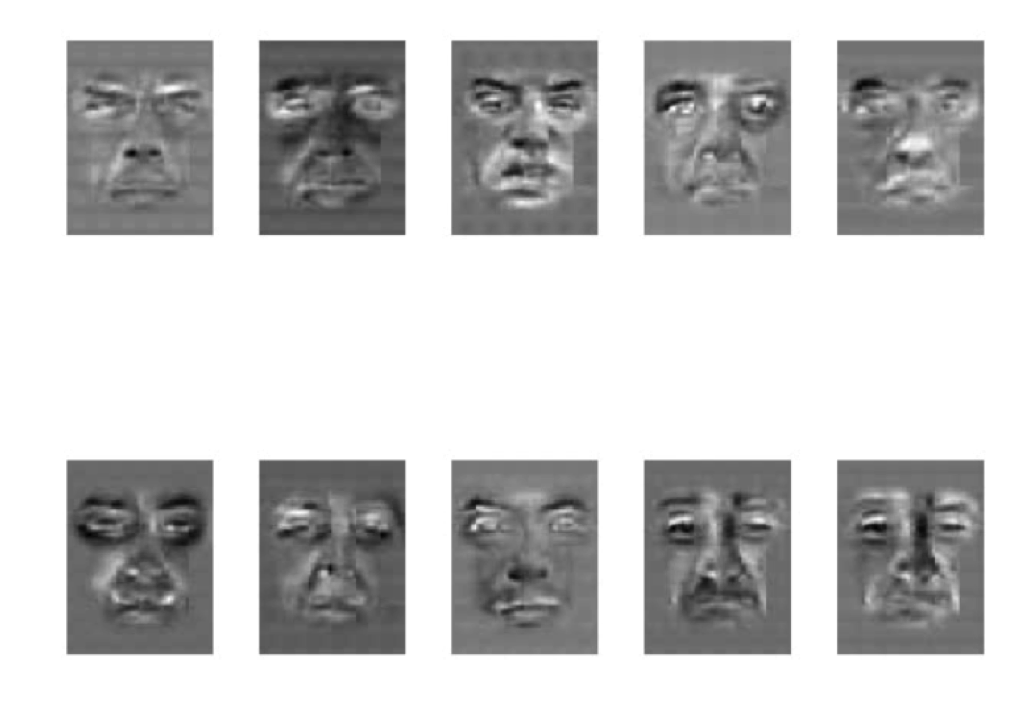
\includegraphics[width=0.65\textwidth]{disgust}
  \caption{Eigenfaces expressing disgust. Source: Lecture 13, slide 34}
\end{figure}


\section{Linear Discriminant Analysis}
\subsection{PCA vs. LDA}
PCA and LDA are similar in that both reduce the dimensions of a sample. However, PCA projections don't consider the labels of the classes. An alternative approach is to move away from PCA toward an algorithm that is optimal for classification (as opposed to reconstruction). Linear Discriminant Analysis (LDA) finds a projection that keeps different classes far away from each other.
\begin{itemize}
	\item PCA maintains maximum variance.
    \item LDA allows for class discrimination by finding a  projection that maximizes scatter between classes and minimizes scatter within classes.
\end{itemize}

\begin{figure}[H]
  \centering
  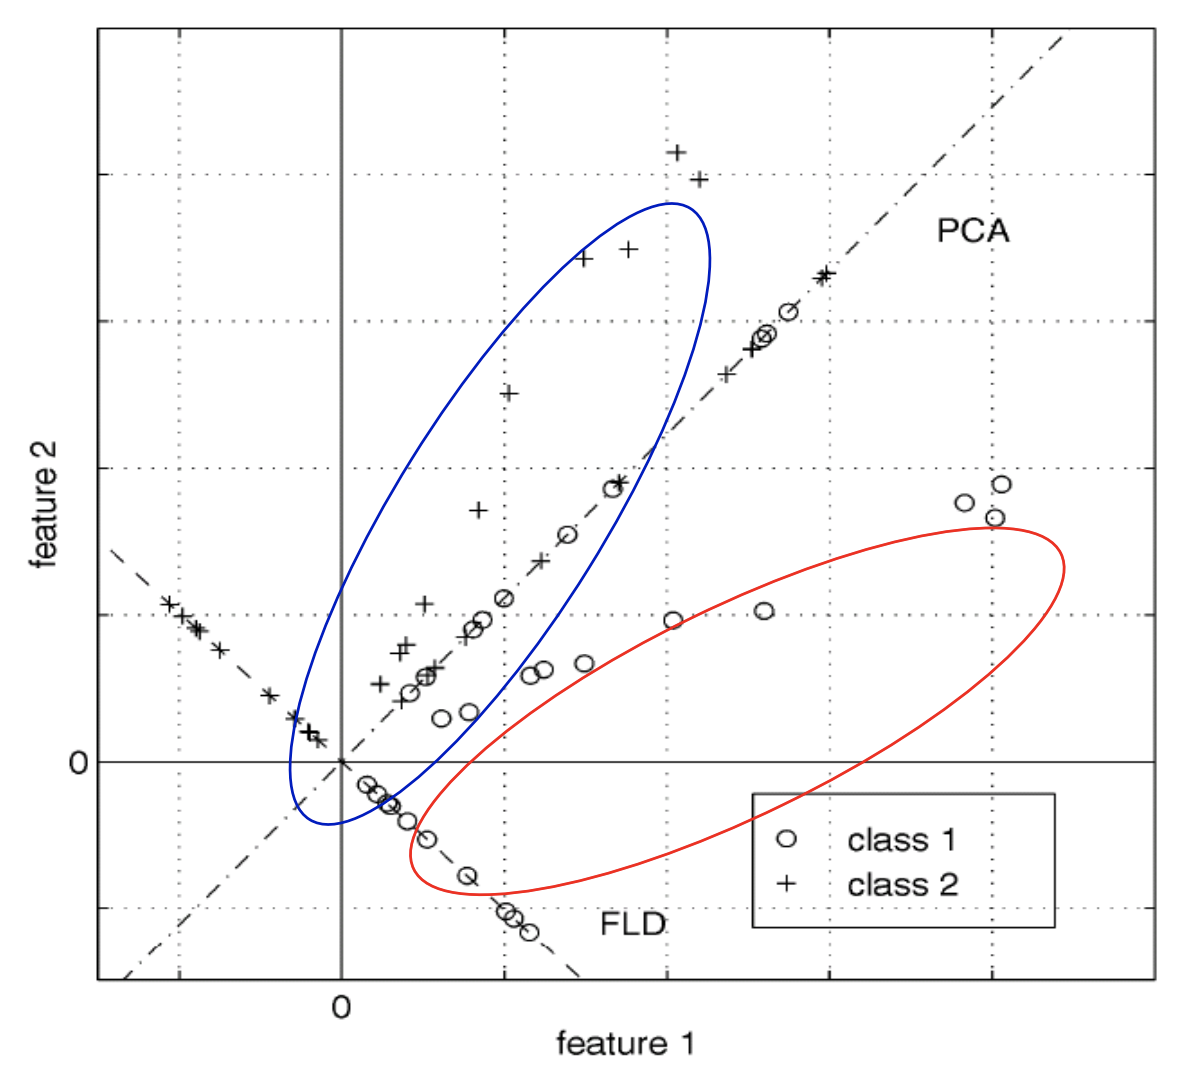
\includegraphics[width=0.65\textwidth]{pca-vs-lda}
  \caption{PCA vs. LDA. Source: Lecture 13, slide 41}
\end{figure}

The difference between PCA and LDA projections is demonstrated in the figure above. PCA preserves the maximum variance and maps the points of the classes along the line with the positive slope, which makes it difficult to distinguish a points' class. Meanwhile, LDA maps the points onto the line with the negative slope, which results in points being located close to other points in their class and far from points in the opposite class.

\subsection{General Idea}

LDA operates using two values: between class scatter and within class scatter. Between class scatter is concerned with the distance between different class clusters, whereas within class scatter refers to the distance between points of a class. LDA maximizes the between-class scatter and minimizes the within-class scatter.

\begin{figure}[H]
  \centering
  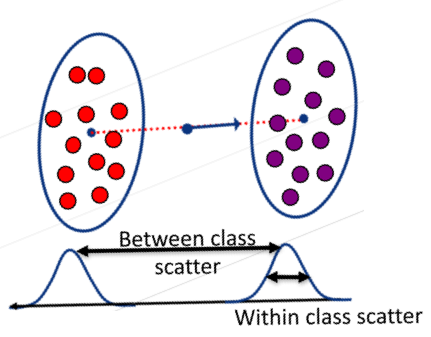
\includegraphics[width=0.65\textwidth]{between-within-scatters}
  \caption{Between Class Scatter vs. Within Class Scatter. Source: Lecture 13, slide 43}
\end{figure}

\subsection{Mathematical Formulation of LDA with 2 Variables}

We want to find a projection $w$ that maps points with classes 0 and 1 in the space $x \in R^n$ to a new space $z \in R^m$, such that $z = w^{T}x$. Ideally, $m < n$, and our projection should maximize the function: 

$$J(w) = \frac{S_B\text{ when projected onto }w}{S_W\text{ when projected onto }w}$$ 

In this equation, $S_B$ represents between class scatter and $S_W$ represents the within-class scatter. Let us then define a variable $\mu_i$ that represents the mean of a class' points:

$$\mu_i = E_{X|Y}[X|Y=i]$$

Let us also define a variable $\Sigma_i$ that represents the covariance matrix of a class: 

$$\Sigma_i = E_{X|Y}[(X-\mu_i)(X-\mu_i)^T|Y=i]$$

Using these values, we can redefine our variables $S_B$ and $S_W$ to be:

$$S_B = (\mu_1-\mu_0)^2 = (\mu_1-\mu_0)(\mu_1-\mu_0)^T$$
$$S_W = (\Sigma_1+\Sigma_0)$$

Plugging these new values of $S_B$ and $S_W$ back into $J(w)$, we get:

$$J(w) = \frac{(\mu_1-\mu_0)^2\text{ when projected onto }w}{(\Sigma_1+\Sigma_0)\text{ when projected onto }w} = \frac{w^T(\mu_1-\mu_0)(\mu_1-\mu_0)^Tw}{w^T(\Sigma_1+\Sigma_0)w}$$ 

We can maximize $J(w)$ by maximizing the numerator, $w^T(\mu_1-\mu_0)(\mu_1-\mu_0)^Tw$, and keeping its denominator, $w^T(\Sigma_1+\Sigma_0)w$ constant. In other words:

$$\text{max }w^T(\mu_1-\mu_0)(\mu_1-\mu_0)^Tw\text{ subject to }w^T(\Sigma_1+\Sigma_0)w = K$$

Using Lagrange multipliers, we can define the Lagrangian as:

$$L = w^TS_Bw-\lambda(w^TS_Ww-K) = w^T(S_B-\lambda S_W)w+K$$

We must then maximize L with respect to $\lambda$ and $w$. We can do so by taking its gradient with respect to $w$ and finding where the critical points are:

$$\nabla_wL = 2(S_B-\lambda S_W)w = 0$$

Using this equation, we get that the critical points are located at:

$$S_Bw = \lambda S_Ww$$

This is a generalized eigenvector problem. In the case where $S_W^{-1} = (\Sigma_1 + \Sigma_0)^{-1}$ exists, we obtain:

$$S_W^{-1}S_Bw = \lambda w$$

We can then plug in our definition of $S_B$ to get:

$$S_W^{-1}(\mu_1-\mu_0)(\mu_1-\mu_0)^Tw = \lambda w$$

Notice that $(\mu_1-\mu_0)^Tw$ is a scalar, and thus we can represent it by a term $\alpha$ such that:

$$S_W^{-1}(\mu_1-\mu_0) = \frac{\lambda}{\alpha} w$$

The magnitude of $w$ does not matter, so we can represent our projection $w$ as:

$$w* = S_W^{-1}(\mu_1-\mu_0) = (\Sigma_1-\Sigma_0)^{-1}(\mu_1-\mu_0)$$


\subsection{LDA with N Variables and C Classes}
\subsubsection{Preliminaries}
\textbf{Variables:}
\begin{itemize}
	\item N sample images: $\{x_1, \cdots, x_N\}$
    \item C classes: $\{Y_1, Y_2, \cdots, Y_C\}$. Each of the N sample images is associated with one class in $\{Y_1, Y_2, \cdots, Y_C\}$.
    \item Average of each class: the mean for class $i$ is $\mu_i = \frac{1}{N_i} \displaystyle\sum_{x_k \in Y_i}x_k$ 
    \item Average of all data: $\mu = \frac{1}{N} \displaystyle\sum_{k=1}^{N}x_k$
\end{itemize}
\textbf{Scatter Matrices:}
\begin{itemize}
	\item Scatter of class $i$: $S_i = \displaystyle\sum_{x_k \in Y_i} (x_k - \mu_i)(x_k - \mu_i)^T$
    \item Within class scatter: $S_w = \displaystyle\sum_{i=1}^{c} S_i$
    \item Between class scatter: $S_b = \displaystyle\sum_{i=1}^{c} N_i(\mu_i-\mu)(\mu_i-\mu)^T$
\end{itemize}

\subsubsection{Mathematical Formulation}
We want to learn a projection $W$ such that it converts all the points from $x\in \mathbb{R}^m$ to a new space $z\in \mathbb{R}^n$, where in general $m$ and $n$ are unknown:
$$z = w^Tx, x\in \mathbb{R}^m, z\in \mathbb{R}^n$$
After the projection, the between-class scatter is $\widetilde{S}_B = W^TS_BW$, where $W$ and $S_B$ are calculated from our original dataset. The within-class scatter is $\widetilde{S}_W = W^TS_WW$. So the objective becomes: 
$$W_{opt} = \argmax_W \frac{\left|\widetilde{S}_B\right|}{\left|\widetilde{S}_W\right|} = \argmax_W \frac{\left|W^TS_BW\right|}{\left|W^TS_WW\right|}$$
Again, after applying Lagrange multipliers we obtain a generalized eigenvector problem, where we have:
$$S_B w_i = \lambda_iS_Ww_i, i = 1, \dots, m$$

Note that $\Rank(S_B)$ and $\Rank(S_W)$ are limited by the number of classes ($C$) and the number of sample images ($N$):
$$\Rank(S_B) \leq C-1$$
$$\Rank(S_W) \leq N-C$$
And therefore the rank of $W_{opt}$ is limited as well.

\subsection{Results: Eigenface vs. Fisherface}
\textit{Belhumeur, Hespanha, Kriegman} performed an experiment comparing the recognition error rates of PCA to LDA ("Eigenface vs Fisherface") using a dataset of 160 images of 10 distinct people. The images contained significant variation in lighting, facial expressions, and eye-wear. Error rates were determined using the "leaving-one-out" strategy, where a single image was classified by removing that image from the dataset and training on the other 159 images, at which point classification was done on the left-out image with a nearest-neighbors classifier. This process was repeated over all 160 images in order to determine an error rate \cite{EigenfacesvsFisherfaces}.

\begin{figure}[H]
  \centering
  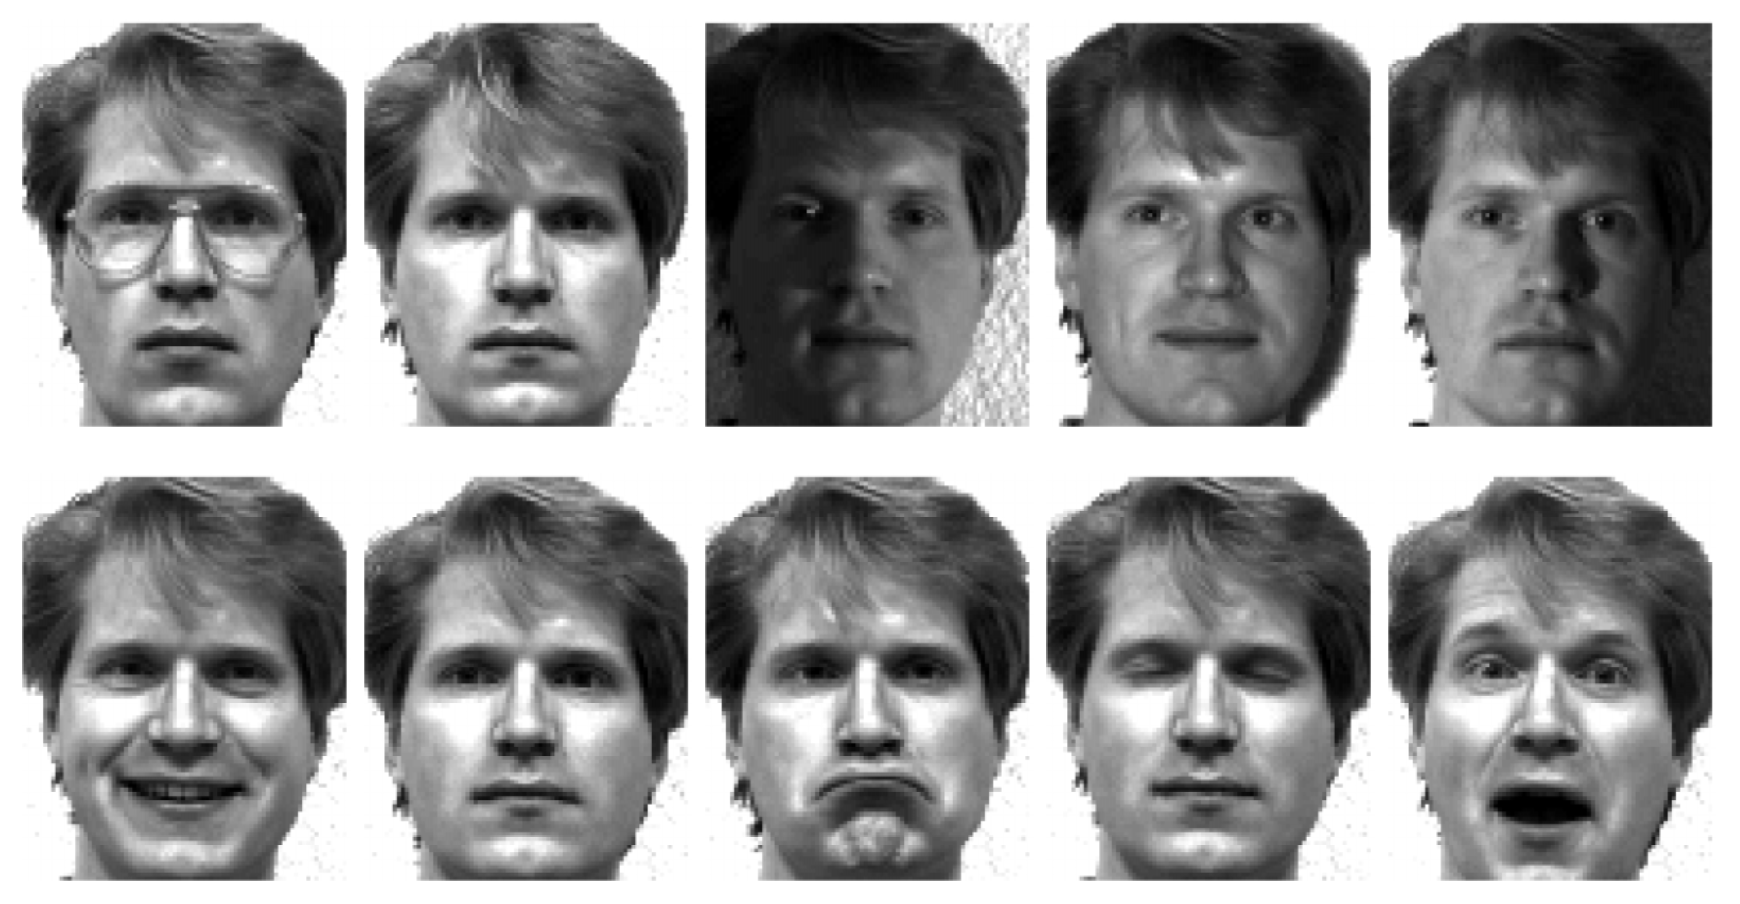
\includegraphics[width=0.7\textwidth]{variation_in_expression}
  \caption{Variation in Facial Expression, Eyewear, and Lighting. Source: \cite{EigenfacesvsFisherfaces}}
\end{figure}

\begin{figure}[H]
  \centering
  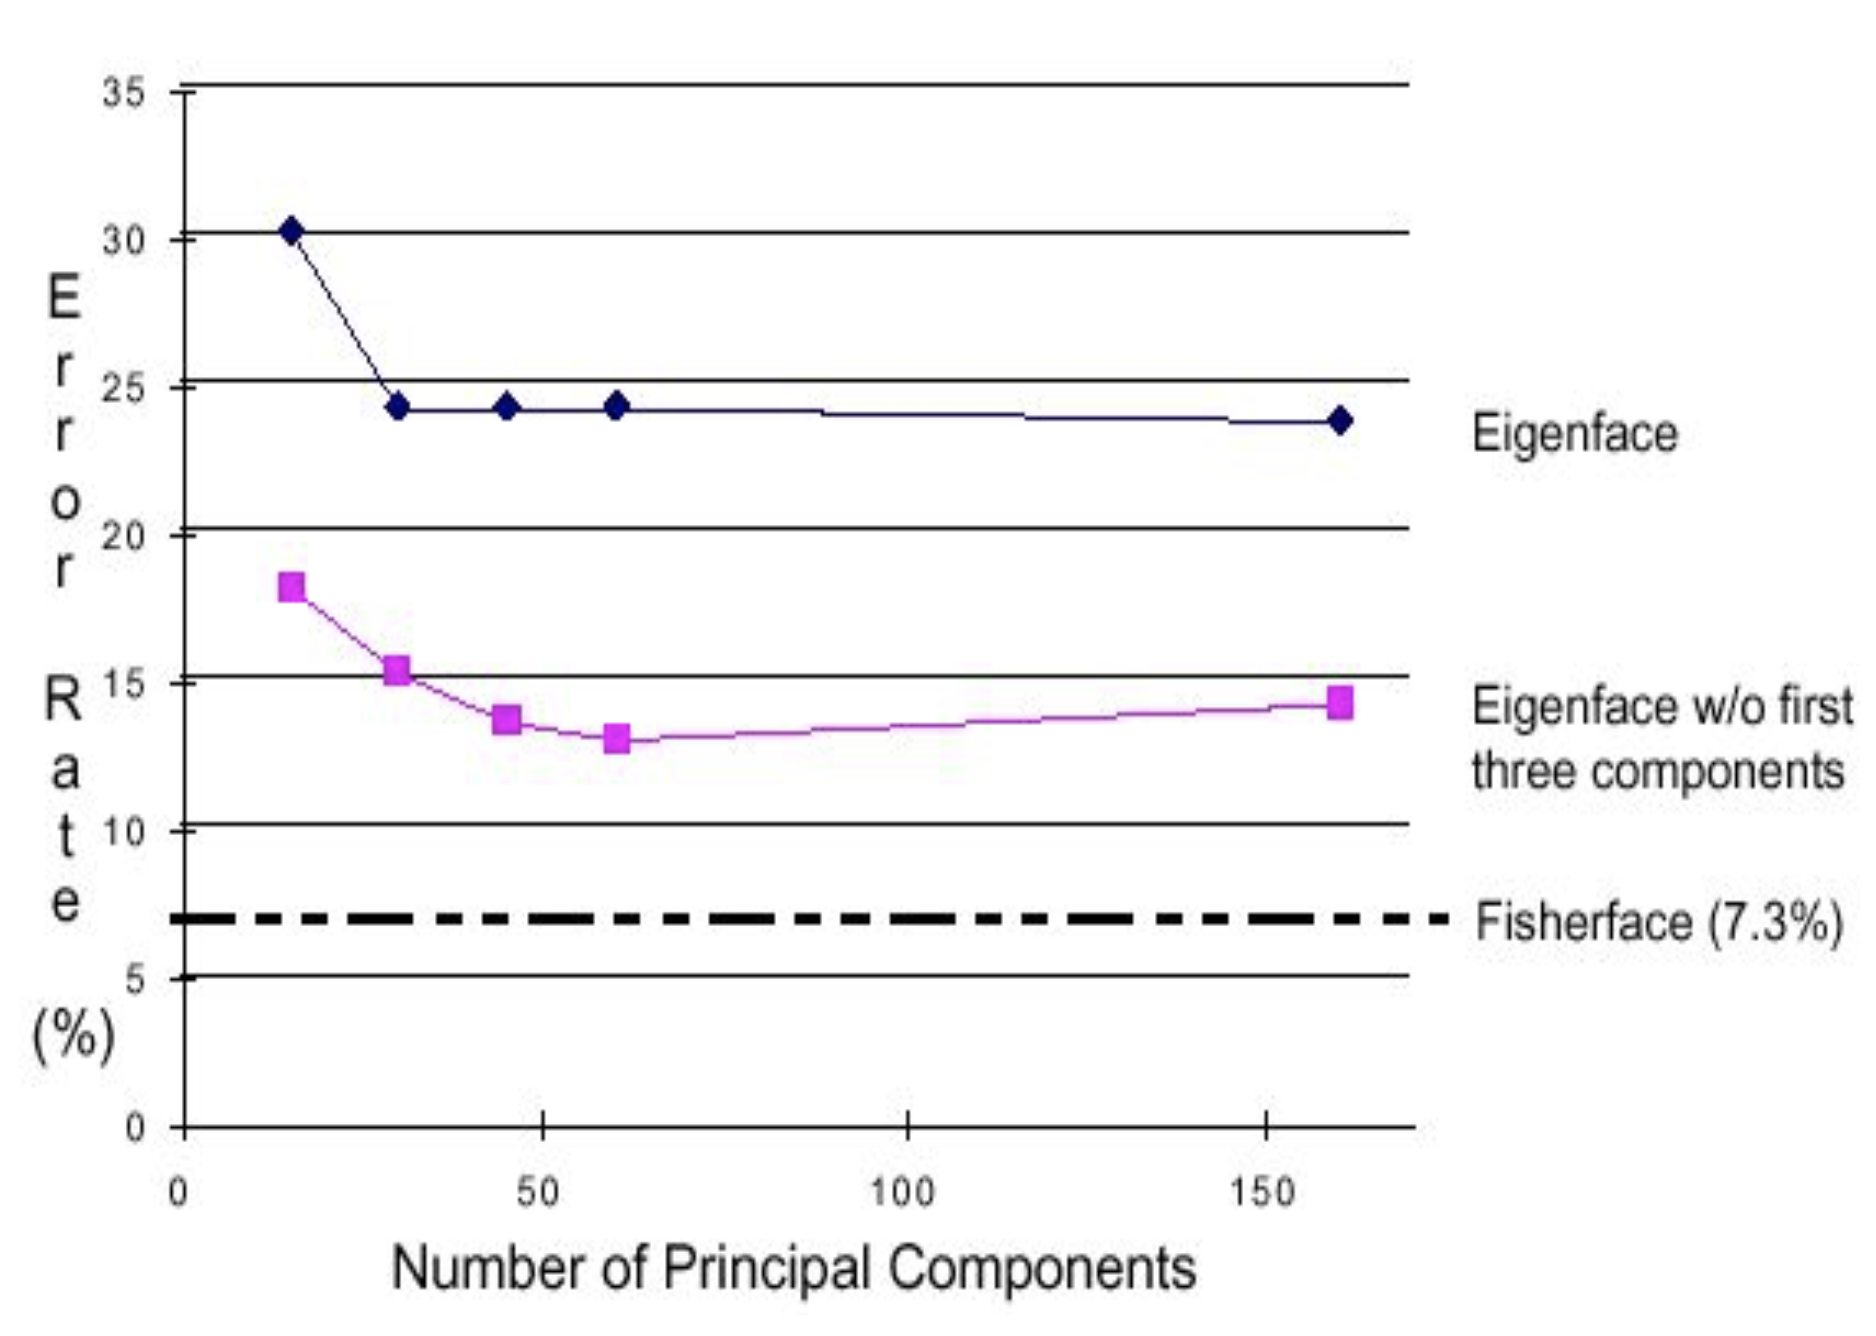
\includegraphics[width=0.8\textwidth]{error_rate}
  \caption{Eigenface vs. Fisherface. Source: Lecture 13, slide 61}
\end{figure}

Error rates for the two algorithms (and a variation of standard Eigenface) are plotted in the figure above. Eigenface's error rate actually improves by removing the first three principle components. Fisherface, as shown in the figure above, gives the lowest error rate.


\small
\bibliographystyle{plain}
\bibliography{sample}

\end{document}